In this section, we describe the user interface of our application. The interface is designed to be intuitive and user-friendly, allowing users to easily navigate through the various features and functionalities of BBP.

Given the nature of BBP, the user interface is user-friendly, providing easy access to all the features and functionalities.

\subsection*{Pages and Navigation}

The application is structured into several pages to ensure a logical user flow and an intuitive experience. 

The following pages represent the core architecture of the platform:

\begin{itemize}
    \item \textbf{Login and Register Page:} Handles user authentication and registering, allowing users to securely access their accounts or create new ones.
    \item \textbf{Home Page:} Serves as the primary dashboard for users, for inserting and starting registering trips and visualizing recent activities.
    \item \textbf{Search Page:} Enables users to search for published routes on the map with all information about the trip.
    \item \textbf{Your Trips Page:} A central hub for managing personal travel plans, displaying both upcoming itineraries and historical booking data.
    \item \textbf{Account Page:} Dedicated to user profile management, where individuals can update personal information, adjust security settings, and manage application preferences.
\end{itemize}

Apart from the Login and Register Page, that is the first page you encounter when opening the application the first time, after the login all other pages are accessible via a bottom navigation bar, allowing users to switch between them easily.

\subsection{Login and Register Page}

\begin{figure}[H]
    \centering
    \begin{minipage}{0.3\linewidth}
        \centering
        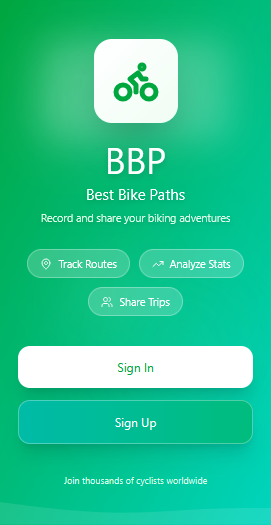
\includegraphics[width=\linewidth]{Images/4-UI.png}
        \caption{Initial Page}
        \label{fig:ui-4}
    \end{minipage}
    \hfill
    \begin{minipage}{0.3\linewidth}
        \centering
        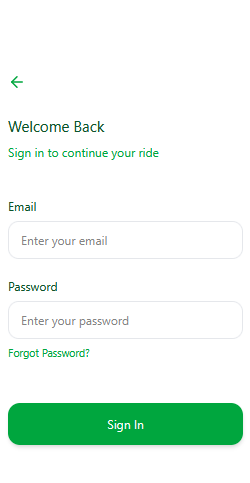
\includegraphics[width=\linewidth]{Images/5-UI.png}
        \caption{Login Page}
        \label{fig:ui-5}
    \end{minipage}
    \hfill
    \begin{minipage}{0.3\linewidth}
        \centering
        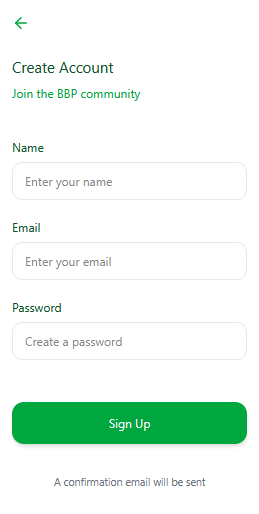
\includegraphics[width=\linewidth]{Images/6-UI.png}
        \caption{Register Page}
        \label{fig:ui-6}
    \end{minipage}
\end{figure}

The first page when you're not logged in is shown in Figure \ref{fig:ui-4}, where you can choose to log in or register a new account.

If you choose to log in, you will be directed to the Login Page shown in Figure \ref{fig:ui-5}, where you can enter your credentials to access your account.

If you don't have an account yet, you can click on the "Sign Up" button to be directed to the Register Page shown in Figure \ref{fig:ui-6}, where you can create a new account by providing the required information.

\subsection{Home Page}

\begin{figure}[H]
    \centering
    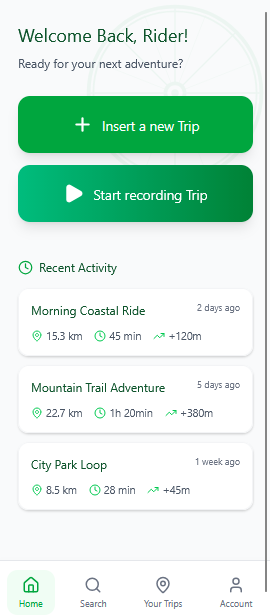
\includegraphics[width=0.35\textwidth]{Images/7-UI.png}
    \caption{Home Page}
    \label{fig:ui-7}
\end{figure}

The Home Page, shown in Figure \ref{fig:ui-7}, serves as the main dashboard for users. 

Here, users can manually insert a trip by clicking on the "Insert a new Trip" button, that will open a form that user have to compile to submit the trip, or start the automatic recording of a new trip by clicking on the "Start recording Trip" button, which will guide them through the trip registration process. 

Additionally, the Home Page displays recent activities and updates related to the user's account.

\subsection{Search Page}

\begin{figure}[H]
    \centering
    \begin{minipage}{0.35\linewidth}
        \centering
        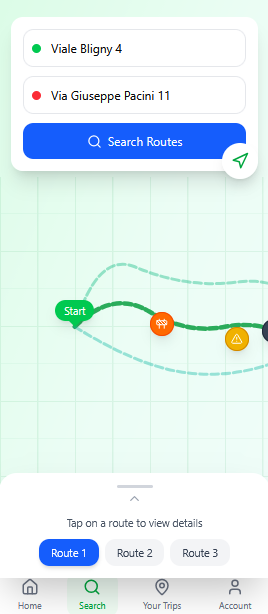
\includegraphics[width=\linewidth]{Images/8-UI.png}
        \caption{Search Page}
        \label{fig:ui-8}
    \end{minipage}
    \hspace{3cm}
    \begin{minipage}{0.35\linewidth}
        \centering
        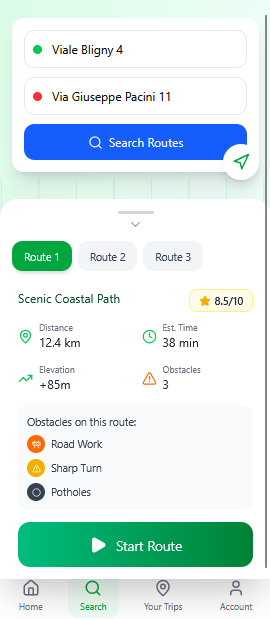
\includegraphics[width=\linewidth]{Images/9-UI.png}
        \caption{Route Details}
        \label{fig:ui-9}
    \end{minipage}
\end{figure}

The Search Page, shown in Figure \ref{fig:ui-8}, allows users to search for published routes on the map inserting start and end point in the forms on the upper part of the page and clicking on them on the map to view detailed information about each trip, as illustrated in Figure \ref{fig:ui-9}.

\subsection{Your Trips Page}

\begin{figure}[H]
    \centering
    \begin{minipage}{0.35\linewidth}
        \centering
        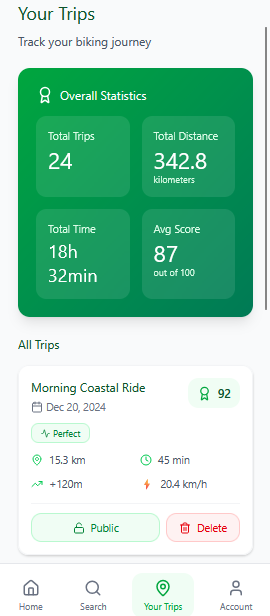
\includegraphics[width=\linewidth]{Images/10-UI.png}
        \caption{Your Trips Page}
        \label{fig:ui-10}
    \end{minipage}
    \hspace{3cm}
    \begin{minipage}{0.35\linewidth}
        \centering
        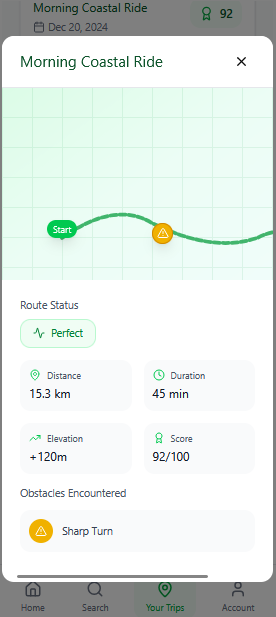
\includegraphics[width=\linewidth]{Images/11-UI.png}
        \caption{Trip Details}
        \label{fig:ui-11}
    \end{minipage}
\end{figure}

The Your Trips Page, shown in Figure \ref{fig:ui-10}, is where users can manage their personal travel plans. It displays both upcoming itineraries and historical booking data. By clicking on a specific trip, users can view detailed information about that trip, as shown in Figure \ref{fig:ui-11}.

\subsection{Account Page}

\begin{figure}[H]
    \centering
    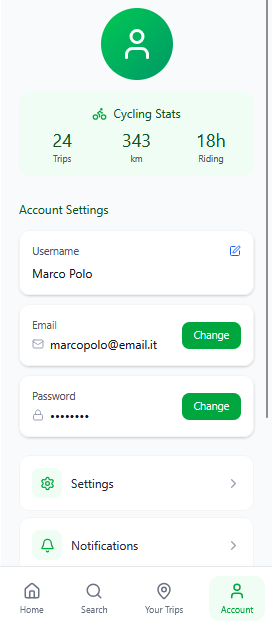
\includegraphics[width=0.35\textwidth]{Images/12-UI.png}
    \caption{Account Page}
    \label{fig:ui-12}
\end{figure}

The Account Page, shown in Figure \ref{fig:ui-12}, is dedicated to user profile management. 

Here, users can update their personal information like name, email, and password and manage application preferences according to their needs.